\documentclass{article}

% Language setting
% Replace `english' with e.g. `spanish' to change the document language
\usepackage[english]{babel}

% Set page size and margins
% Replace `letterpaper' with `a4paper' for UK/EU standard size
\usepackage[letterpaper,top=2cm,bottom=2cm,left=3cm,right=3cm,marginparwidth=1.75cm]{geometry}

\setlength{\parskip}{1em}
\usepackage{listings}

% Useful packages
\usepackage{amsmath}
\usepackage{graphicx}
\usepackage[colorlinks=true, allcolors=blue]{hyperref}
\usepackage{makecell, multirow, tabularx} % pack for table
\newcolumntype{C}{>{\centering\arraybackslash}X} % for centering
\usepackage{float}%for pic to follow words
\usepackage{ctex}% change abstract name
\ctexset{
abstractname = {Statement}
}

\title{MATH6005--Assignment 1}
\author{Chenxuan Sun}
\author{u7983176}
\begin{document}
	\maketitle
	\begin{abstract}
		The assignment I have submitted has been produced according to the rules on Page 1 of Assignment 1. The solutions produced have been written/typed on my own. I have not used AI to prepare my solutions. I have provided references of sources I have used when appropriate.
		\centering Student ID: u7983176
	\end{abstract}
	\newpage

	% question 1.A
\documentclass[options]{class}	\section{Question 1}
		\textbf{Part A}
		\noindent	
			Q: Write a statement form in disjunctive normal form that corresponds to the input-output table below. Draw a diagram of a logic circuit using this statement form.\\
		\textbf{Answer 1.A}
		\begin{table*}[h]
			\centering
			\caption{Q1.A} 
			\label{tab:T1A} 
			\begin{tabularx}{\textwidth}{|C|C|C|C|} 
				\hline
				X & Y & Z & Output \\
				\hline 
				1 & 1 & 1 & 0 \\
				\hline 
				1 & 1 & 0 & 0 \\
				\hline 
				1 & 0 & 1 & 0 \\
				\hline 
				0 & 1 & 1 & 1 \\
				\hline 
				1 & 0 & 0 & 1 \\
				\hline 
				0 & 1 & 0 & 1 \\
				\hline 
				0 & 0 & 1 & 0 \\
				\hline 
				0 & 0 & 0 & 0 \\
				\hline
			\end{tabularx}
		\end{table*}
		
		\begin{figure}[H]
			\centering
			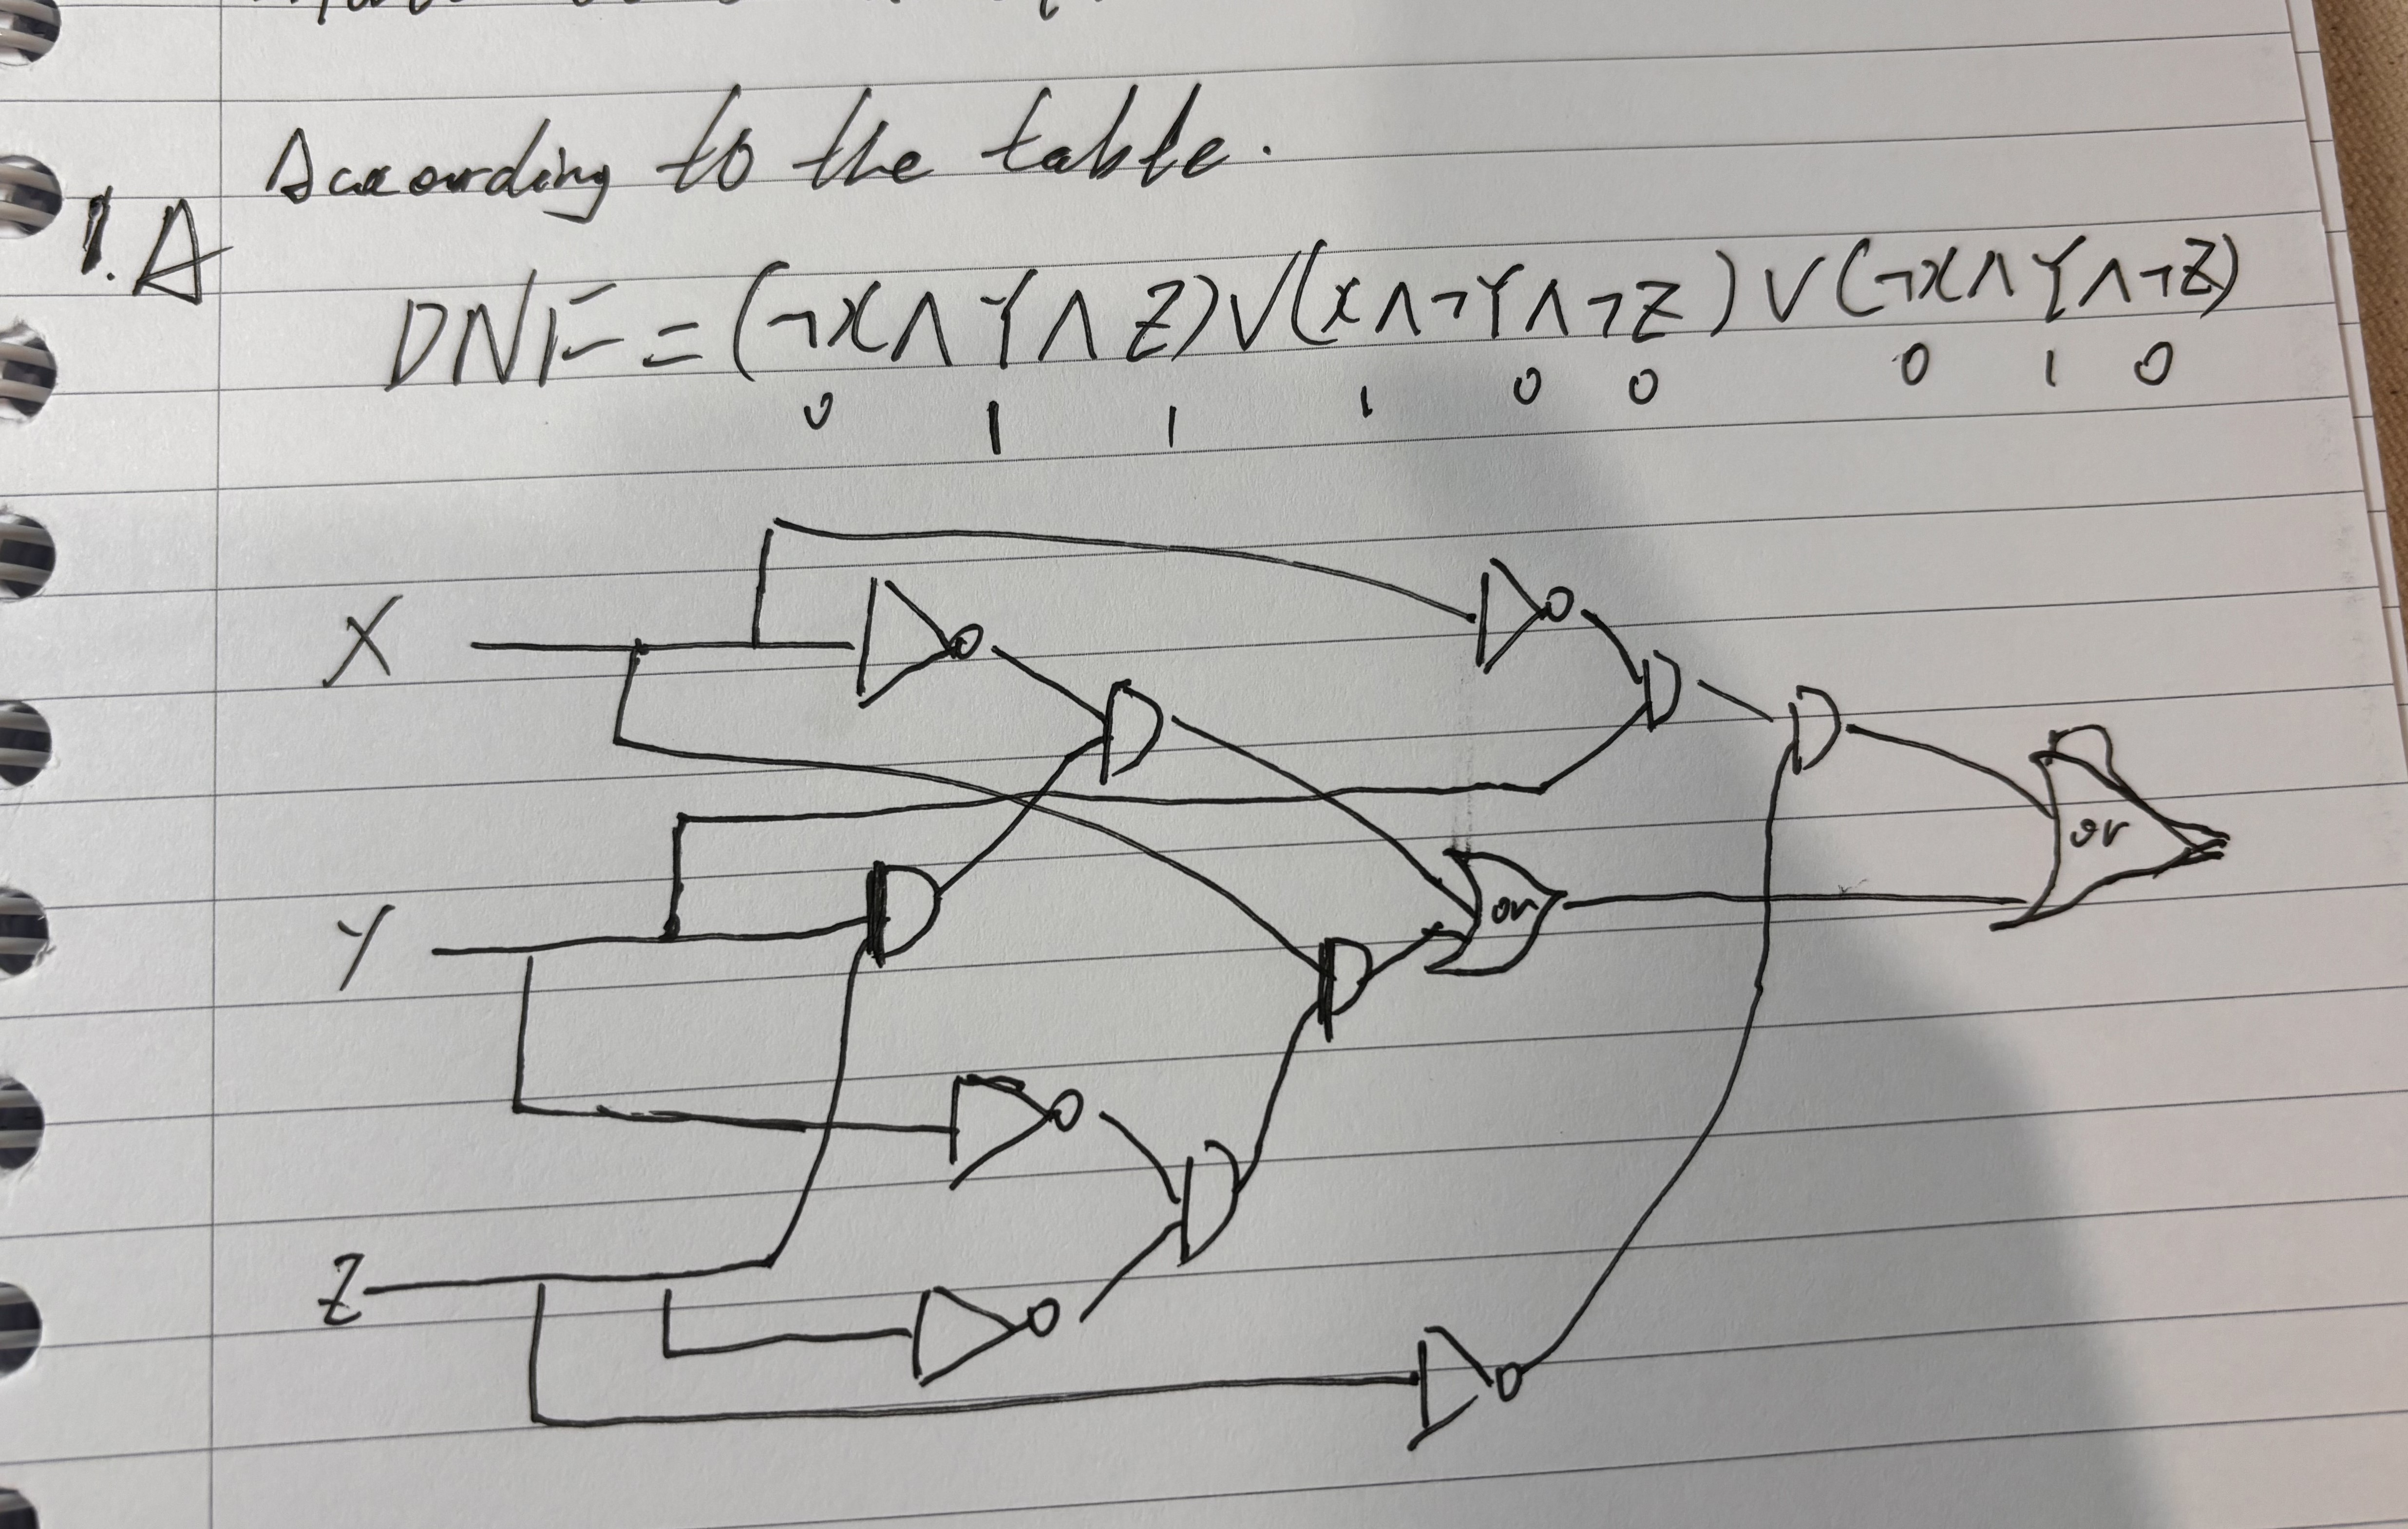
\includegraphics[width=0.75\linewidth]{1.A.jpg}
			\caption{Written answer for Q1.A}
		\end{figure}
		\newpage
		
		% question 1.B
		\textbf{Part B}
		\noindent	
		{Q: Define the logical connective NOR, denoted by X ↓ Y , with the following truth table:}\\
		\textbf{I} Show that X ↓ X ≡ ¬X.\\
		\textbf{et of connectives.\\II} Determine whether the following statement is true or false, and explain your reasoning:\\
		The set {↓} is a functionally complete s
		You can use results from lectures, but must reference them clearly.\par
		
		
		\noindent
		\textbf{Answer 1.B.I}: Since the truth tables agree, they are constantly equal.\par
		\begin{table*}[h]
			\centering
			\caption{Answer: 1.B} 
			\label{tab:T1B} 
			\begin{tabularx}{\textwidth}{|C|C|C|} 
				\hline
				X & X↓X & ¬X \\
				\hline 
				1 & 0 & 0 \\
				\hline 
				0 & 1 & 1 \\
				\hline
			\end{tabularx}
		\end{table*}
		
		\noindent
		\textbf{Answer 1.B.II}: \\
		True. According to Lecture 2\cite{ref1}, it has been proved that:\\
		The set {$\wedge, \vee, \neg$} is a functionally complete set of logical connectives.\\
		Since, \\
		$¬X = X↓X$\\
		$X\wedge Y = ¬(X↓Y )= (X↓Y)↓(X↓Y)$\\
		$X\vee Y = (X↓X)↓(Y↓Y)$\\
		Thus, the NOR operation can be used to conduct completely functional sets of logical operations. the set \(\{\downarrow\}\) is functionally complete.\par
		
		
		% question 1.C
		\textbf{Part C}
		\noindent	
		{Q:Let p(x), q(y) and r(z) be predicates with domains Dp, Dq and Dr respectively. Let the negations of these predicates be}\\
			$p′(x) ≡ ¬p(x), q′(y) ≡ ¬q(y) and r′(x) ≡ ¬r(x).$\\
		Consider the statement:\\
			$∀x ∈ Dp ∃y ∈ Dq ∀z ∈ Dr (p(x) → (q(y) ∧ r(z)))$\\
		Take the the negation of this statement. By using logical equivalences, express the negated statement so that ‘¬’ no longer appears. Explain each step (you can reference logical equivalences from lecture slides).

		\newpage
		\noindent
		\textbf{Answer 1.C}:
		\begin{figure}[H]
			\centering
			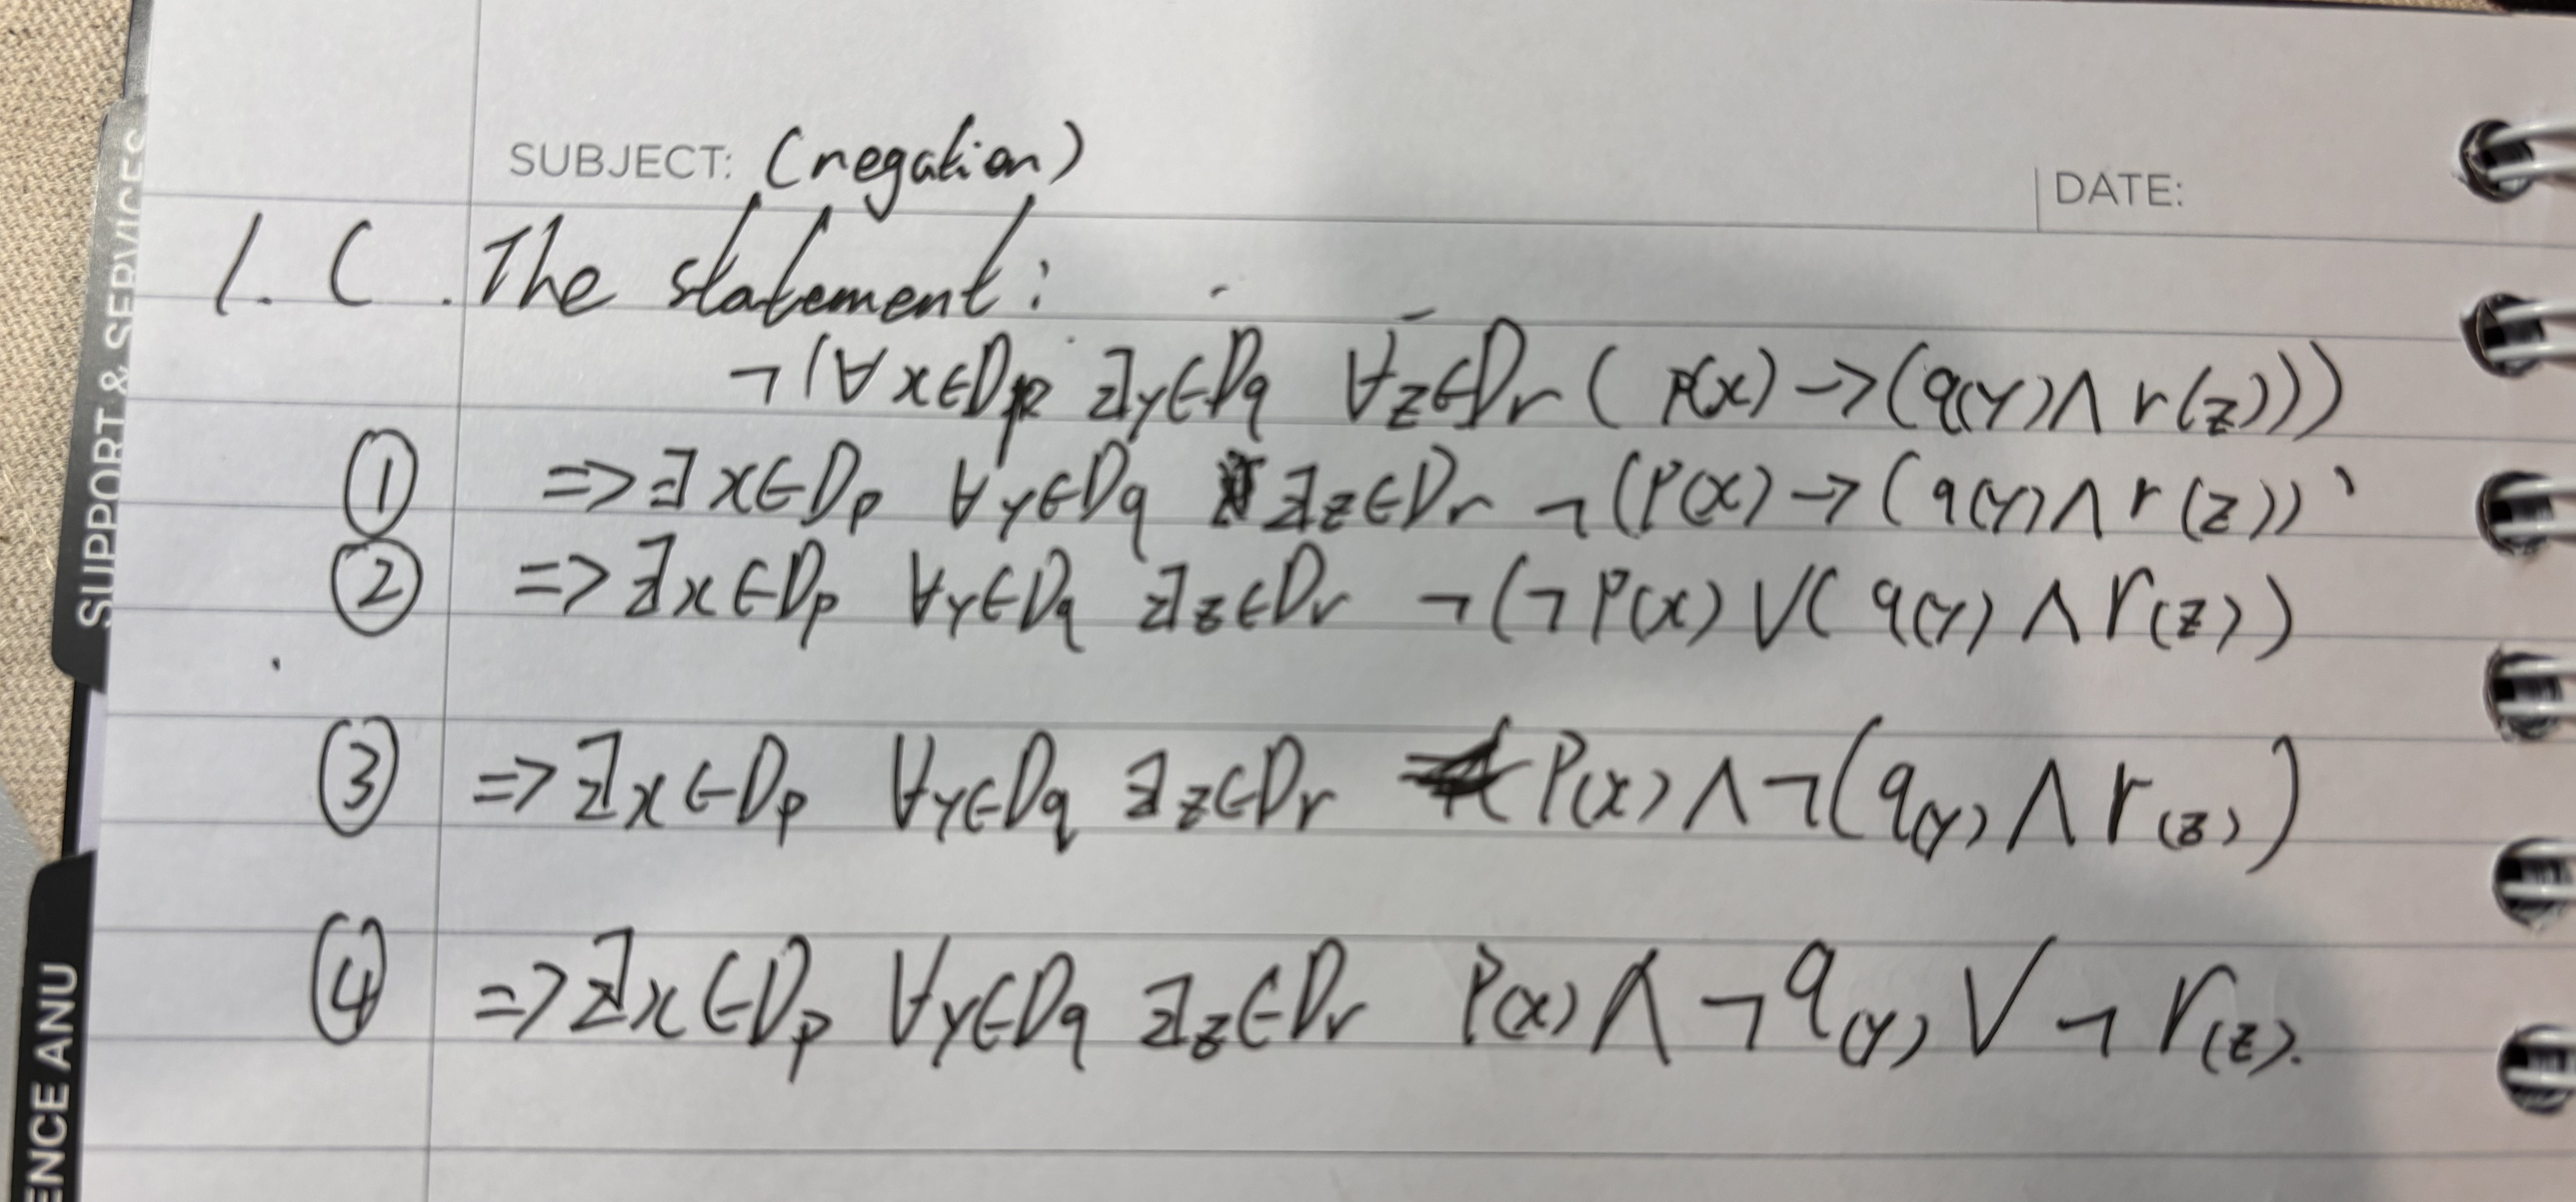
\includegraphics[width=0.75\linewidth]{1.C.jpg}
			\caption{Written answer for Q1.C}
		\end{figure}
		
		\noindent
		\textbf{Step1:} According to the rule of negation of quantifiers: \\
			¬∀xP(x)≡∃x¬P(x) AND ¬∃xP(x)≡∀x¬P(x)\\
		\textbf{Step2:} According to \\
			p→q≡¬p∨q\\
		\textbf{Step 3 \& 4:} According to De Morgan's laws, remove parentheses and toggle logical symbols within parentheses.\par
		
		Therefore, 
		Further processing of each negation symbol:\\
		\begin{center}
		$¬q(y)≡q′(y)$\\
		$¬r(z)≡r′(z)$\\
		\end{center}
		\[
		\exists x \in D_p \, \forall y \in D_q \, \exists z \in D_r \, \big(p(x) \land (q'(y) \lor r'(z))\big)
		\]
		\newpage
		
	% question 2
	\section{Question 2}
	%2.A
	\textbf{Part A}
		\noindent	
		Q:Let A, B and C be subsets of a universal set U. Prove that:\\
			(A ∩ B) ∪ C = (A ∪ C) ∩ (B ∪ C).
			
		\par
		\noindent
		\textbf{Answer 2.A}: the logical equivalences:
		
		\begin{figure}[H]
			\centering
			\includegraphics[width=0.75\linewidth]{2.A.EQUAL.jpg}
			\caption{the logical equivalences table for Q2.A}
		\end{figure}
		\par
		
		\par
		\noindent
		\textbf{Answer 2.A}: the proof process
		
		\begin{figure}[H]
			\centering
			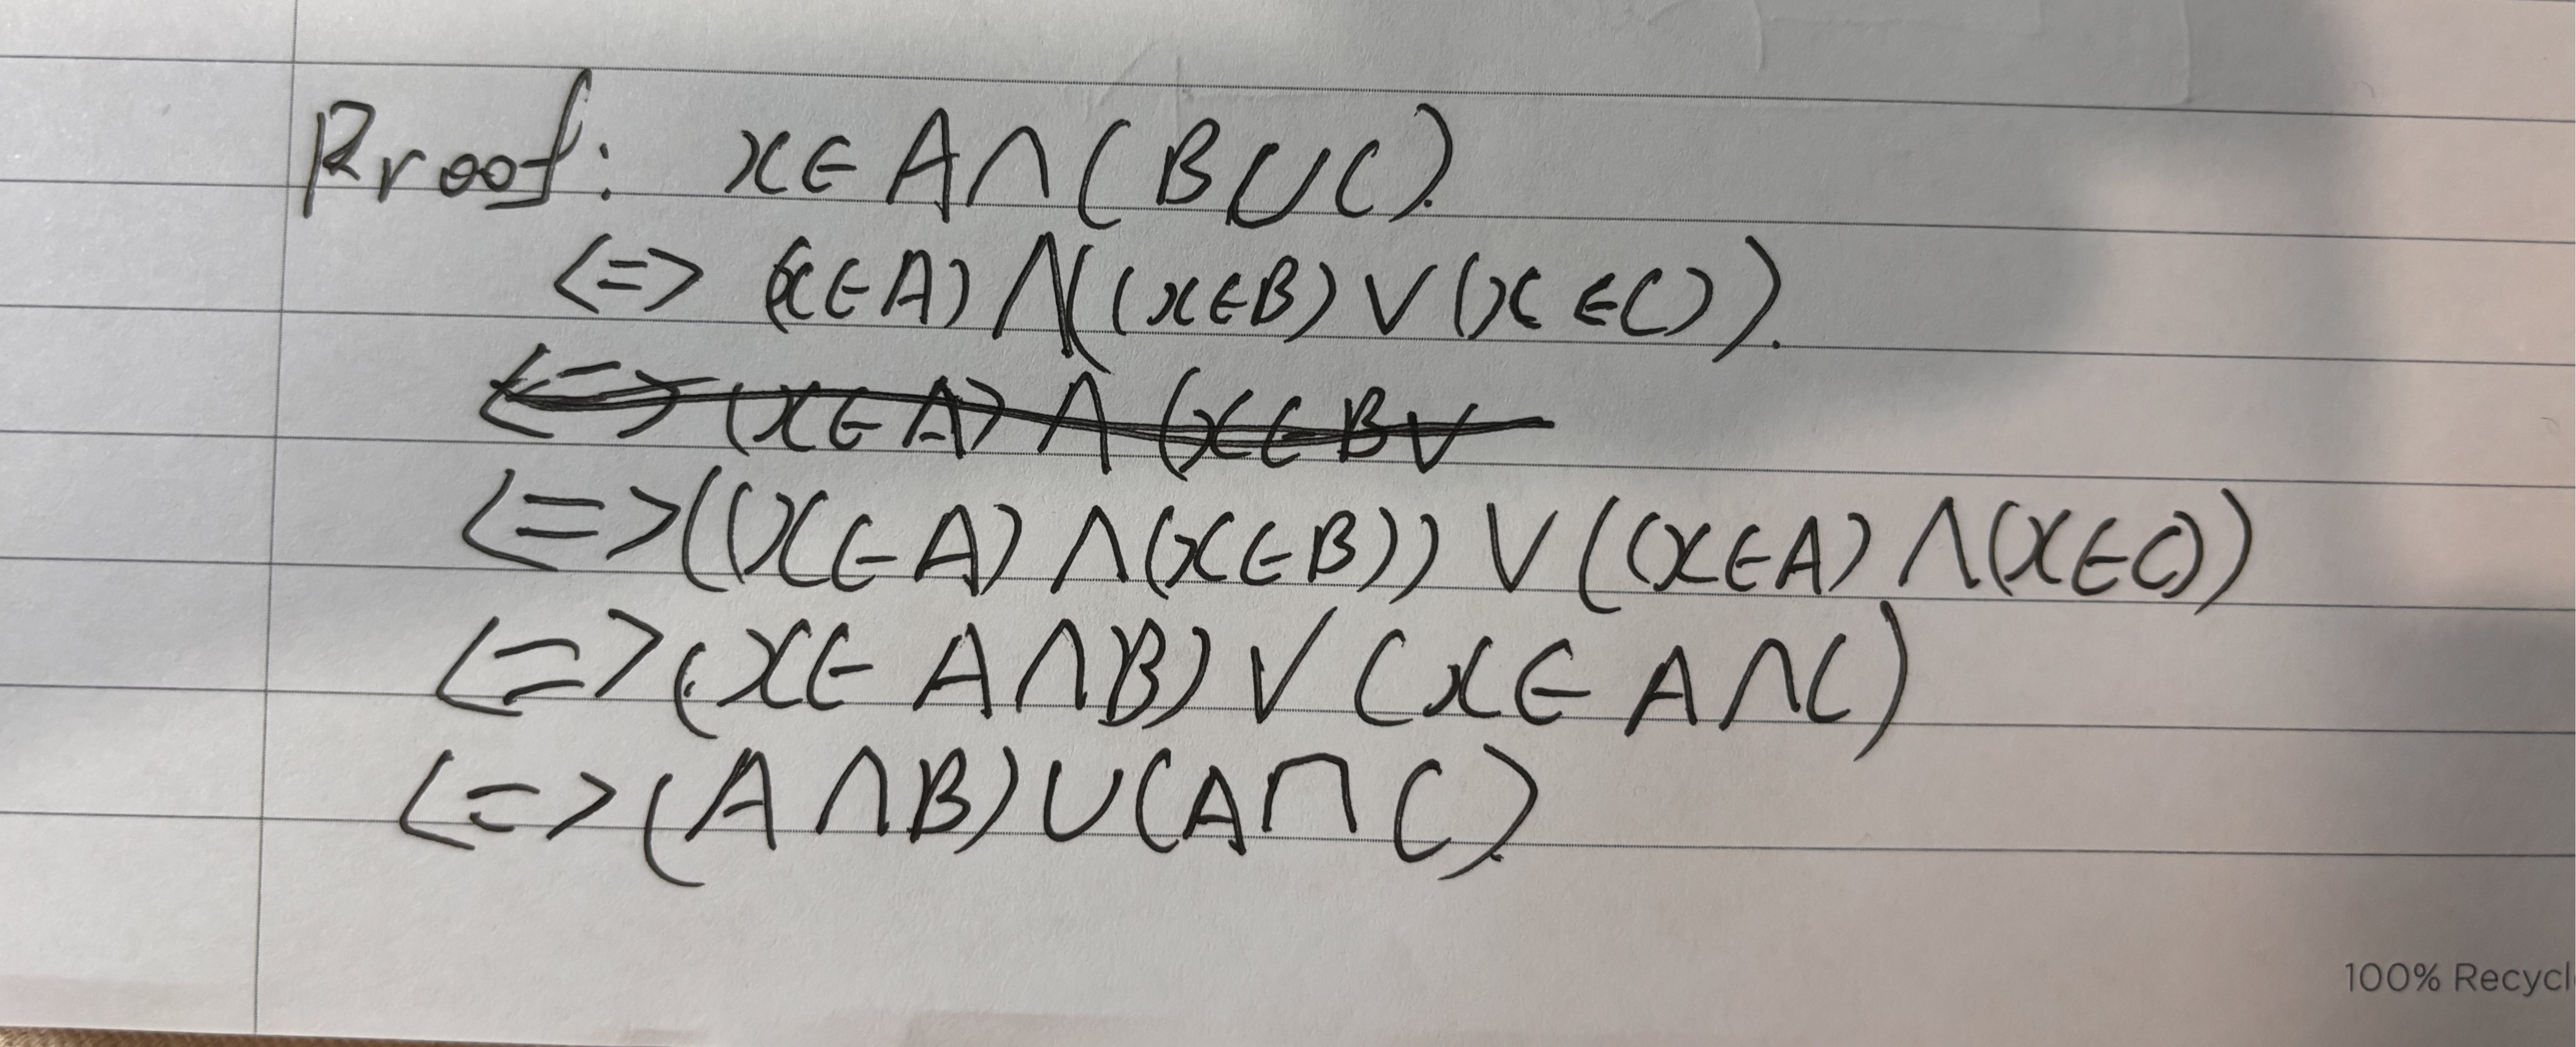
\includegraphics[width=0.75\linewidth]{2.A.PROOF.jpg}
			\caption{Proof for Q2.A}
		\end{figure}
		The combination of the above truth table and the argumentation process shows that the equation holds true.
		\par
		
		\newpage
		
	%2.B
	\textbf{Part B}
		\noindent	
		Q: Let A = {a} and X = {v, x}.
			\textbf{I}
			List all the possible relations from A to X:\\
			
			\begin{center}
				R1= \{ $\emptyset$ \}\\ 
				R2= \{(a,x)\}\\
				R3 = \{(a,y)\}\\
				R4= \{(a,x),(a,y)\}\\ 
			\end{center}
			\textbf{II}
			
			\par
			\noindent	
			Since the function's condition is ∀a ∈ A ∃!b ∈ B (a, b) ∈ f,\\
			The R1 doesn't exist a codomain;\\
			R4 exist two elements for the \{a\} in set A;\\
			only R2 and R3 has only one element for \{a\}.\\
			Therefore, only R2 and R3 are functions.\\
			\par
			
	%2.C
	\textbf{Part C}
		\noindent	
		Q: Let B = {c, d} and Y = {y, z}.
		\textbf{I}
		List all the possible functions with domain B and codomain Y \\
		
		\begin{center}
			f1 = \{(c, y),(d, y)\} \\
			f2 = \{(c, y),(d, z)\} \\
			f3 = \{(c, z),(d, z)\} \\
			f4 = \{(c, z),(d, y)\} \\
		\end{center}
		
		\textbf{II}
		For each function found in part C.I, state whether the function is bijective or not. In each case, justify your answer carefully.\\
		\noindent	
		The function f2 and f4 is injective;\\
		The function f2 and f4 is surjective;\\
		Therefore, f2 and f4 are bijective.\\
		\noindent
		f3 and f4 are not injective because {c} has 2 different outputs;\\
		f3 and f4 are not bijective because the codomain is not fully mapped.\\ 
		\par
		
		\newpage
	% question 3
	\section{Question 3}
	\subsection*{What is a Pseudorandom Number Generator (PRNG)?}
	A pseudorandom number generator (PRNG) is a tool that produces a sequence of numbers that appear random, but are actually generated by a specific mathematical process. Unlike a true random number generator, which relies on unpredictable physical processes, a PRNG uses a defined formula and a starting point, called a seed, to generate numbers. This allows PRNGs to produce repeatable sequences of numbers if the same seed is used.
	\subsubsection*{Example:How Does a Linear Congruential Generator (LCG) Work?}
	A Linear Congruential Generator (LCG) is a simple type of PRNG that uses the following formula to generate numbers:
	\[
	X_{n+1} = (aX_n + c) \mod m
	\]
	where:
	\(X_n\) is the current number,\(X_{n+1}\) is the next number,\(a\) is a constant multiplier,\(c\) is a constant increment,\(m\) is the modulus, or maximum value,\(n\) is the current step in the sequence.
	This formula takes the current number \(X_n\), multiplies it by \(a\), adds \(c\), and then takes the remainder when dividing by \(m\). The result is the next number in the sequence, \(X_{n+1}\).
	\subsection*{Advantages of Using PRNGs Over True Random Number Generators}
	Comparing to a true random number generator, PRNGs have following advantages, including: reproducibility, fast and efficient in generating, control over sequence characteristics like length and distribution, and the easy implement without needing specialized hardware.
	\subsubsection*{Example:Why LCGs Provide the Advantages of PRNGs}
	\begin{itemize}
		\item \textbf{Easy to Implement}: The LCG algorithm requires minimal code and can be easily implemented in any programming language.
		\item \textbf{Fast and Efficient}: LCGs use only a few arithmetic operations to generate each number, making them very fast.
		\item \textbf{Reproducibility}: Because LCGs are deterministic, using the same seed will always produce the same sequence. 
		\item \textbf{Long Periods and Good Distribution}: With carefully chosen parameters (\(a\), \(c\), and \(m\)), LCGs can generate long sequences of numbers with good distribution properties, meaning the numbers appear random and are evenly spread out.
	\end{itemize}

	\newpage
	
	% question 4
	\section{Question 4}
	
	\textbf{Part A}
	
	\textit{Q:} Find all of the companions of 7. Justify your answer.
	
	\textit{Answer:} \\
	to qualify \( g = 1, 2, 3, 4, 5, 6 \) 
	
	\begin{itemize}
		\item \( g = 1 \):
		\[
		1^1 = 1, \quad 1^2 = 1, \quad 1^3 = 1, \quad 1^4 = 1, \quad 1^5 = 1, \quad 1^6 = 1
		\]
		the set is \(\{1\}\) , not the companion of 7.
		
		\item \( g = 2 \):
		\[
		2^1 = 2, \quad 2^2 = 4, \quad 2^3 = 8 \equiv 1 \pmod{7}, \quad 2^4 = 16 \equiv 2 \pmod{7}, \quad 2^5 = 32 \equiv 4 \pmod{7}, \quad 2^6 = 64 \equiv 1 \pmod{7}
		\]
		the set is  \(\{1, 2, 4\}\),not the companion of 7.
		
		\item \( g = 3 \):
		\[
		3^1 = 3, \quad 3^2 = 9 \equiv 2 \pmod{7}, \quad 3^3 = 27 \equiv 6 \pmod{7}, \quad 3^4 = 81 \equiv 4 \pmod{7}, \quad 3^5 = 243 \equiv 5 \pmod{7}, \quad 3^6 = 729 \equiv 1 \pmod{7}
		\]
		the set is \(\{1, 2, 3, 4, 5, 6\}\) ,is the companion of 7.
		
		\item \( g = 4 \):
		\[
		4^1 = 4, \quad 4^2 = 16 \equiv 2 \pmod{7}, \quad 4^3 = 64 \equiv 1 \pmod{7}, \quad 4^4 = 256 \equiv 4 \pmod{7}, \quad 4^5 = 1024 \equiv 2 \pmod{7}, \quad 4^6 = 4096 \equiv 1 \pmod{7}
		\]
		the set is \(\{1, 2, 4\}\) , not the companion of 7.
		
		\item \( g = 5 \):
		\[
		5^1 = 5, \quad 5^2 = 25 \equiv 4 \pmod{7}, \quad 5^3 = 125 \equiv 6 \pmod{7}, \quad 5^4 = 625 \equiv 2 \pmod{7}, \quad 5^5 = 3125 \equiv 3 \pmod{7}, \quad 5^6 = 15625 \equiv 1 \pmod{7}
		\]
		the set is \(\{1, 2, 3, 4, 5, 6\}\) ,is the companion of 7.
		
		\item \( g = 6 \):
		\[
		6^1 = 6, \quad 6^2 = 36 \equiv 1 \pmod{7}, \quad 6^3 = 216 \equiv 6 \pmod{7}, \quad 6^4 = 1296 \equiv 1 \pmod{7}, \quad 6^5 = 7776 \equiv 6 \pmod{7}, \quad 6^6 = 46656 \equiv 1 \pmod{7}
		\]
		the set is  \(\{1, 6\}\) , not the companion of 7.
	\end{itemize}
	
	\par
	\par
	
	\textbf{Part B}
	
	\textit{Q:} Describe how you would go about proving or disproving the following statement: 104651 is prime and 24576 is a companion of 104651.
	
	\textit{Answer:}
	
	To determine if the number 104651 is prime, the most straightforward way is to divide ( n ) by all integers from 2 up to the square root of ( n ).\\
	Here is the code with python.
	\begin{lstlisting}
		% coding with python
		def is_prime(n):
			if n <= 1:
				return False
			if n <= 3:
				return True 
			if n % 2 == 0 or n % 3 == 0:
				return False
			i = 5
			while i * i <= n:
				if n % i == 0 or n % (i + 2) == 0:
					return False
				i += 6 
				# Skip all even numbers and numbers divisible by 3.
				
			return True
	\end{lstlisting}
	
	To prove :  24576 is a companion of 104651.\\
	The code is :
	\begin{lstlisting}
	def is_companion(g, p):
		found = set()
		for a in range(1, p):
			found.add(pow(g, a, p))
		return found == set(range(1, p))
		return True
	\end{lstlisting}
	\par
	\par
	Based on the two codings blocks, \\
	
	\begin{lstlisting}
	104651 is a prime number: True
	24576 is a companion of 104651: True
	\end{lstlisting}
	\par 
	\par 
	
	
	\textbf{Part C}
	
	\textit{Q:} Let p = 104651, g = 24576 and s = 100418. Compute g
	s mod p using Steps (1)-(4), showing all your working. In your working you should never compute or write down a number that exceeds p\^2.
	
	\textit{Answer:} \\
	My draft is the picture below:
	\begin{figure}[H]
		\centering
		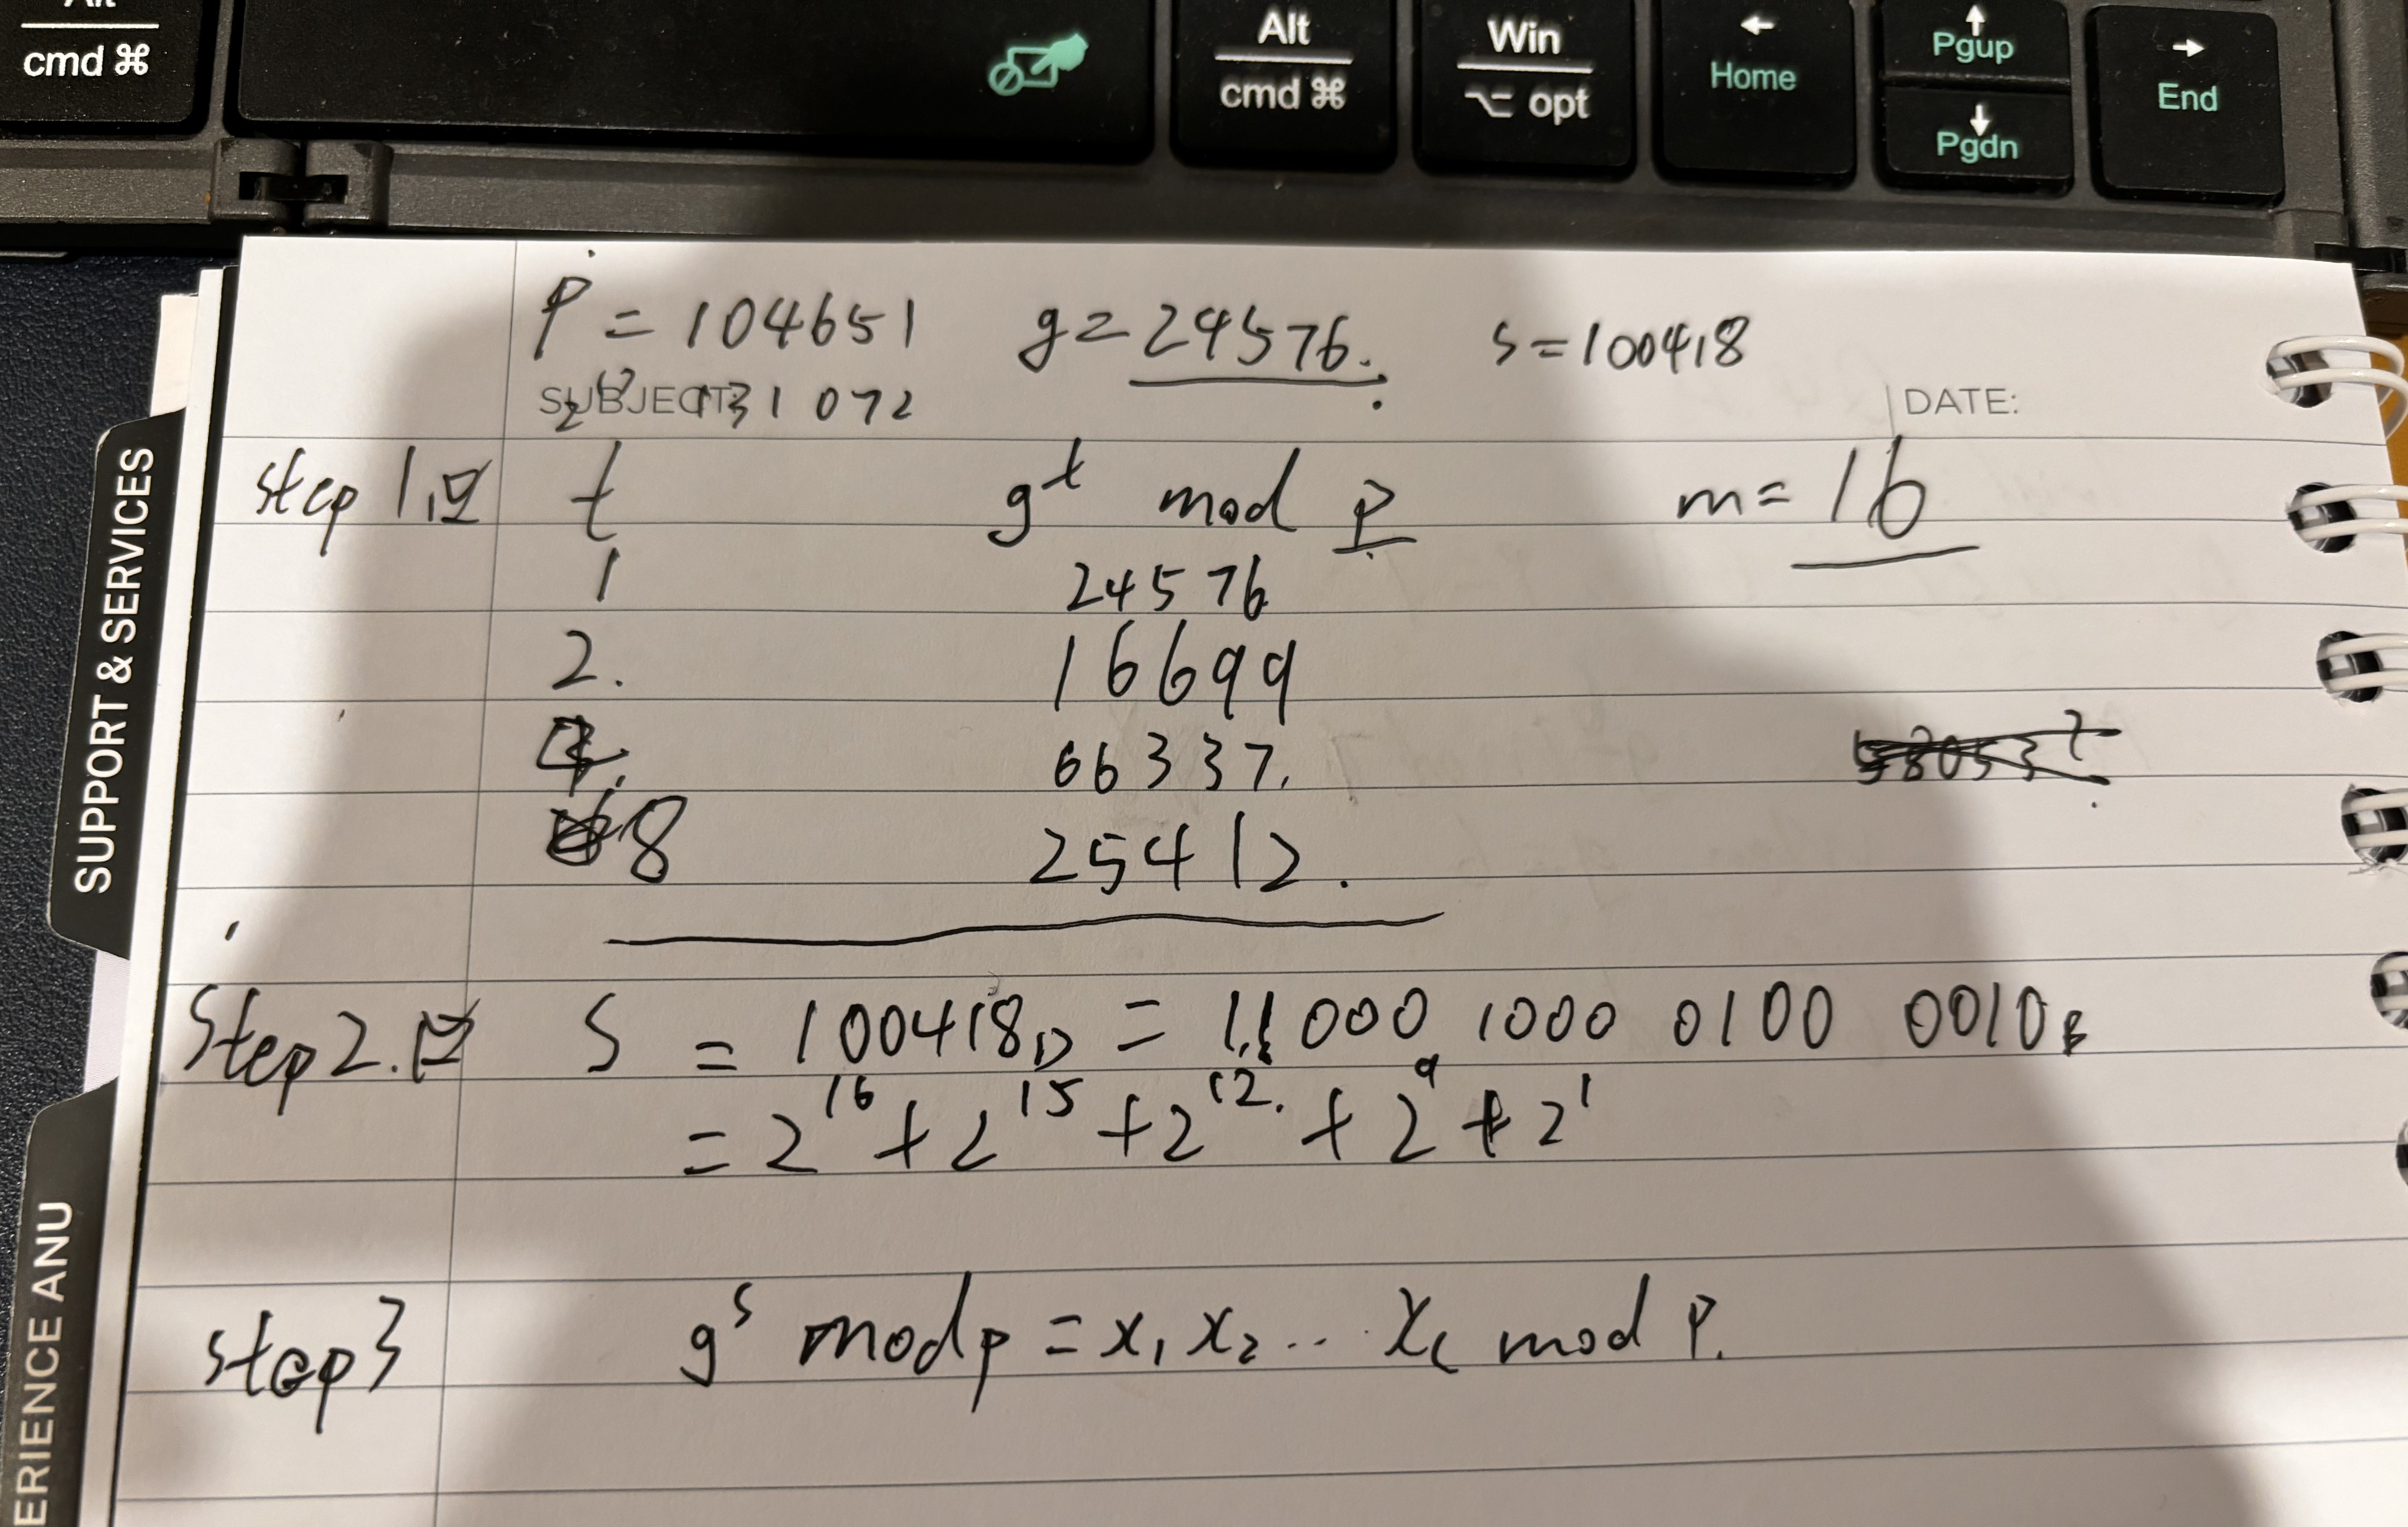
\includegraphics[width=0.75\linewidth]{4c.jpg}
		\caption{Draft for Q4.c}
	\end{figure}
	
	the code is showed below:
	
	\begin{lstlisting}
		p = 104651
		g = 24576
		s = 100418
		
		# Step 1: Compute the table of values for t and g^t mod p
		table = {}
		t = 1
		while t <= p:
			table[t] = pow(g, t, p)
			t *= 2
		
		# Step 2: Write s as a sum of powers of 2
		powers_of_two = []
		current_s = s
		while current_s > 0:
			largest_power = current_s.bit_length() - 1
			powers_of_two.append(2 ** largest_power)
			current_s -= 2 ** largest_power
		
		# Step 3: Find the corresponding x_i values from the table
		x_values = [table[power] for power in powers_of_two]
		
		# Step 4: Compute g^s mod p using x_i values
		result = 1
		for x in x_values:
			result = (result * x) % p
		
		# Output final result
		print(f"g^s mod p = {result}")
		
	\end{lstlisting}
	
	\textbf{Therefore,} 
	the output is :
	\begin{lstlisting}
		g^s mod p = 48441
	\end{lstlisting}
	
	\textbf{Part C}

	\textit{Q:} Find s and explain how you found it. You will need to write some form of code to answer this(any language you are familiar with is fine, but you should provide the code and explain how it works). Your method should be efficient and not store a number exceeding p2	(if you uselibrary functions, you must know they do not store a number exceeding p2)
	
	\textit{Answer:} \\
	Given:\\
	p=104651\\
	g=24576\\
	24576 \^ s mod 104651=3190\\
	
	According to the conclusion of part c, s is a binary number formed by matching powers of 2, so can use the same means to find s in reverse.\\
	
	Step 1: The table is created similarly as part c, containing the values g \^t mod p\\

	Step 2: The second part finds the first combination whose product is equal to the target value by generating and checking all power combinations and returns it. The function internally defines an auxiliary function, compute\_product, to compute the product of the power combinations and to take the modulus for p. The arithmetic complexity can be simplified by using the method of summing by bits.\\
	
	\begin{lstlisting}
	# Given values
	p = 104651
	g = 24576
	
	# Step 1: Compute the table of values for t and g^t mod p
	table = {}
	t = 1
	while t <= p:
	table[t] = pow(g, t, p)
	t *= 2
	
	# Output the computed table
	print("Computed table of powers of g modulo p:")
	for power, value in table.items():
	print(f"g^{power} mod p = {value}")
	
	# # Function to find the combination that multiplies to target
	# def find_combination(table, target, p):
	#     powers = list(table.keys())
	#     for r in range(1, len(powers) + 1):
	#         for combo in combinations(powers, r):
	#             product = 1
	#             for power in combo:
	#                 product = (product * table[power]) % p
	#             if product == target:
	#                 return combo
	#     return None
	
	# Target value
	target = 3190
	
	# List of powers in the table
	powers = list(table.keys())
	
	# Function to find combinations of powers that multiply to target
	def find_combination(table, target, powers, p):
	n = len(powers)
	
	# Helper function to compute product modulo p
	def compute_product(combo):
	product = 1
	for power in combo:
	product = (product * table[power]) % p
	return product
	
	# Check all combinations of the powers
	for i in range(1, 2 ** n):
	combo = []
	for j in range(n):
	if (i >> j) & 1:
	combo.append(powers[j])
	
	if compute_product(combo) == target:
	return combo
	return None
	
	# Find the combination
	combo = find_combination(table, target, powers, p)
	
	if combo:
	print(f"The combination of powers of g that equals {target} mod {p} is: {combo}")
	# Calculate the value of s
	s = sum(combo)
	print(f"The value of s is: {s}")
	else:
	print("No combination found.")
	
	\end{lstlisting}
	
	the outputs are:
	\begin{lstlisting}
	
	The combination of powers of g that equals 3190 mod 104651 is: [8, 16, 32, 1024, 4096, 8192, 32768]
	The value of s is: 46136
	\end{lstlisting}	

	\begin{thebibliography}{99}  
		\bibitem{ref1}Townsend K, Discrete Mathematical Models Lecture 2, ANU, 2024 pp23.
		
	\end{thebibliography}
	
\end{document}
